\subsection{Meetopstelling} \label{sec:methods}
In \cref{sec:introduction} is een model beschreven waarmee path loss kan worden gemodelleerd. In dat model wordt er gebruik gemaakt van een fittingscoëfficiënt. Deze fittingscoëfficiënt kan echter anders zijn afhankelijk van de omgeving. Om een indicatie te krijgen van welke waarde de fittingscoëfficiënt heeft in het Jacoba Mulder Huis, zal in dit hoofdstuk een testopstelling worden toegelicht waarmee de fittingscoëfficiënt bepaald zou kunnen worden.

% \subsection{Meetopstelling}
Voor de metingen is gebruik gemaakt van de materialen die in \cref{tab:measurement:materials} staan. Deze materialen zijn volgens \cref{fig:measurementSetup} opgesteld. Hierbij staan beide antennes op een hoogte van 1 meter en in eerste instantie op 1 meter afstand. Vervolgens is er met de signaal generator vanaf -10dBm in stappen van 2dBm tot 4dBm gezonden op een frequentie van 2.4GHz. Per zendniveau is er vervolgens met een spectrumanalyzer gemeten wat het ontvangst vermogen is. Nadat voor al de verschillende zendvermogens het ontvangst vermogen is gemeten, wordt de afstand tussen de antennes vergroot met een meter. 
\begin{table}[ht]
    \centering
    \begin{tabular}{l|l|l}
        Apparaat                            & Serienummer       & Beschrijving \\\hline
        Rigol                               & DSG3B171400069    & Signaalgenerator \\
        Rhode\&Schwarz FSP                  & 100538            & Spectrumanalyzer \\
        BNC kabel                           & n.v.t             & BNC kabel van 1 meter \\
        BNC kabel                           & n.v.t             & BNC kabel van 1 meter \\
        BNC $->$ sma adapter                & n.v.t             & BNC male naar SMA female adapter \\
        BNC $->$ N-type adapter             & n.v.t             & BNC male naar N-type female adapter \\
        2.45GHz antenne ($G_{t/r}=2.5$dBi)  & n.v.t             & 2.45GHz antenne (YGL001AA) \\
        2.45GHz antenne ($G_{t/r}=2.5$dBi)  & n.v.t             & 2.45GHz antenne (YGL001AA) \\\hline
    \end{tabular}
    \caption{Materialen die zijn gebruikt voor de metingen in dit meetrapport}
    \label{tab:measurement:materials}
\end{table}
% place figure of measurement schematic
\begin{figure}[ht]
    \centering
    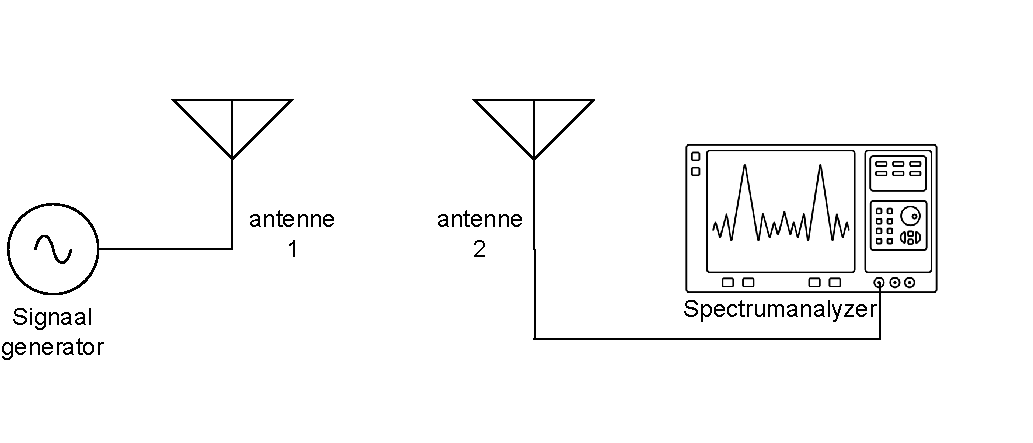
\includegraphics[width=0.7\textwidth]{measurementSetup}
    \caption{De meetopstelling van dit meetrapport.}
    \label{fig:measurementSetup}
\end{figure}

% Description of measurement setup

% Location of measurements

% Table of serial numbers of the used equipement